\section{Increasing System Performance}

\begin{concept}{Performance Optimization Trade-offs}\\
\begin{tabular}{|l|l|}
\hline
\textbf{Optimizing for} & \textbf{Drawbacks on} \\
\hline
Higher speed & Power, cost, chip area \\
\hline
Lower cost & Speed, reliability \\
\hline
Zero power consumption & Speed, cost \\
\hline
Super reliable & Chip area, cost, speed \\
\hline
Temperature range & Power, cost, lifetime \\
\hline
\end{tabular}
\end{concept}

\begin{concept}{Instruction Set Architectures}\\
\textbf{RISC (Reduced Instruction Set Computer):}
\begin{itemize}
  \item Few instructions with uniform format
  \item Fast decoding, simple addressing
  \item Less hardware → higher clock rates
  \item More chip space for registers (up to 256)
  \item Load-store architecture reduces memory access
  \item CPU works at full speed on registers
  \item Enables shorter, efficient pipelines 
\end{itemize}

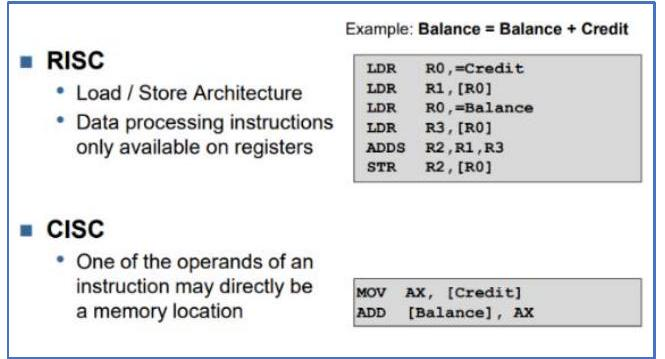
\includegraphics[width=\linewidth]{images/2024_12_29_79e6b22f503fb7b4f718g-13(1)}

\textbf{CISC (Complex Instruction Set Computer):}
\begin{itemize}
  \item More complex instruction set
  \item Lower memory usage for programs
  \item Potential performance gain for short programs
  \item More complex hardware required
\end{itemize}
\end{concept}

\begin{definition}{Computer Architectures}\\
\textbf{Von Neumann Architecture:}
\begin{itemize}
  \item Single memory for program and data
  \item Single bus system between CPU and memory
\end{itemize}

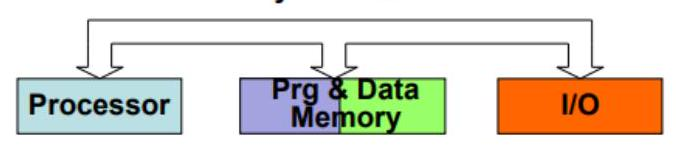
\includegraphics[width=\linewidth]{images/2024_12_29_79e6b22f503fb7b4f718g-13}

\textbf{Harvard Architecture:}
\begin{itemize}
  \item Separate program and data memories
  \item Two sets of address/data buses
  \item Originally from Harvard Mark I
\end{itemize}

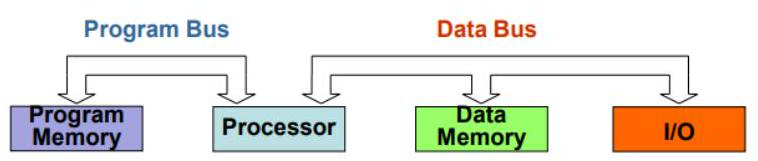
\includegraphics[width=\linewidth]{images/2024_12_29_79e6b22f503fb7b4f718g-13(2)}
\end{definition}

\begin{concept}{Pipelining}\\
Process of fetching next instruction while current one decodes:

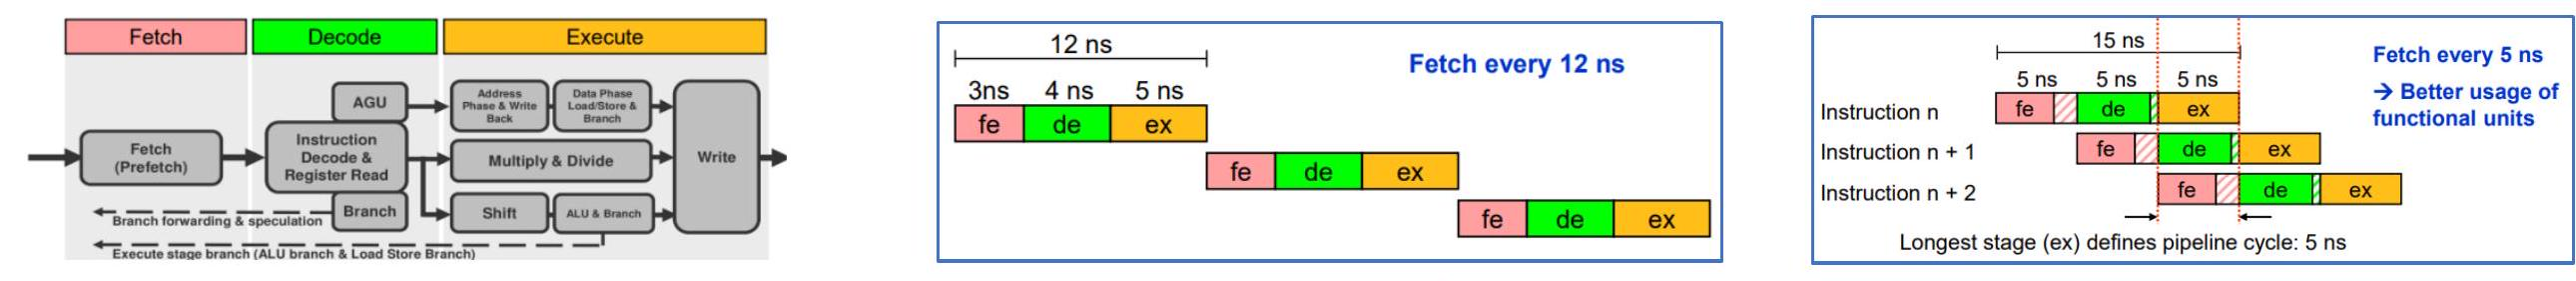
\includegraphics[width=\linewidth]{images/2024_12_29_79e6b22f503fb7b4f718g-14(2)}

\textbf{Pipeline Stages (Example):}
\begin{itemize}
  \item Fetch (Fe): Read instruction - 3ns
  \item Decode (De): Process instruction - 4ns
  \item Execute (Ex): Execute and writeback - 5ns
\end{itemize}

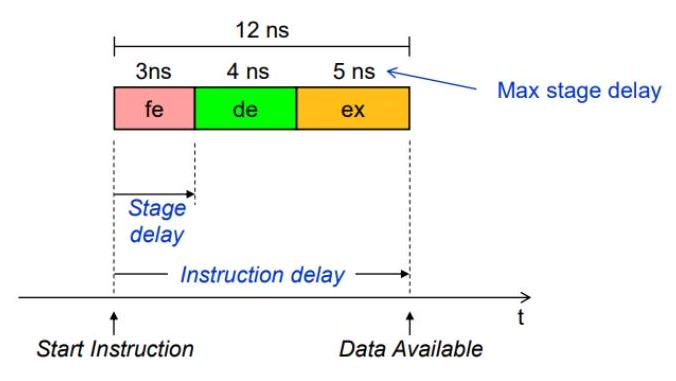
\includegraphics[width=\linewidth]{images/2024_12_29_79e6b22f503fb7b4f718g-14(1)}

\textbf{Advantages:}
\begin{itemize}
  \item Uniform execution time per stage
  \item Significant performance improvement
  \item Simpler hardware per stage
\end{itemize}

\textbf{Disadvantages:}
\begin{itemize}
  \item Blocking stages affect whole pipeline
  \item Memory access conflicts between stages
\end{itemize}
\end{concept}

\begin{definition}{Pipeline Performance}\\
Without pipelining:
\[\frac{\text{Instructions}}{\text{second}} = \frac{1}{\text{Instruction delay}}\]

With pipelining:
\[\frac{\text{Instructions}}{\text{second}} = \frac{1}{\text{Max stage delay}}\]

Note: Pipeline must be filled first
\end{definition}

\begin{example2}{Pipeline Execution}\\
\textbf{Optimal Case:}
\begin{itemize}
  \item Register-only operations
  \item 6 instructions in 6 cycles
  \item CPI = 1 (Cycles Per Instruction)
\end{itemize}

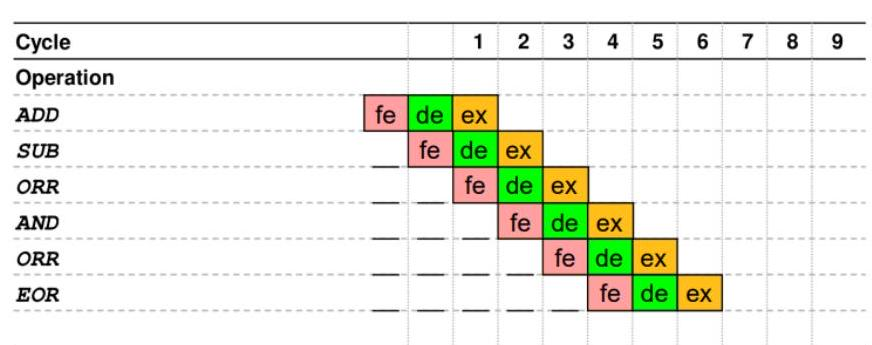
\includegraphics[width=\linewidth]{images/2024_12_29_79e6b22f503fb7b4f718g-14}

\textbf{LDR Special Case:}
\begin{itemize}
  \item 6 instructions in 7 cycles due to memory access
  \item Pipeline stalls for memory read
  \item CPI = 1.2
\end{itemize}
\end{example2}

\begin{concept}{Pipeline Hazards and Optimization}\\
\textbf{Control Hazards:}
\begin{itemize}
  \item Branch decisions in execute stage
  \item Pipeline stalls for taken branches
\end{itemize}

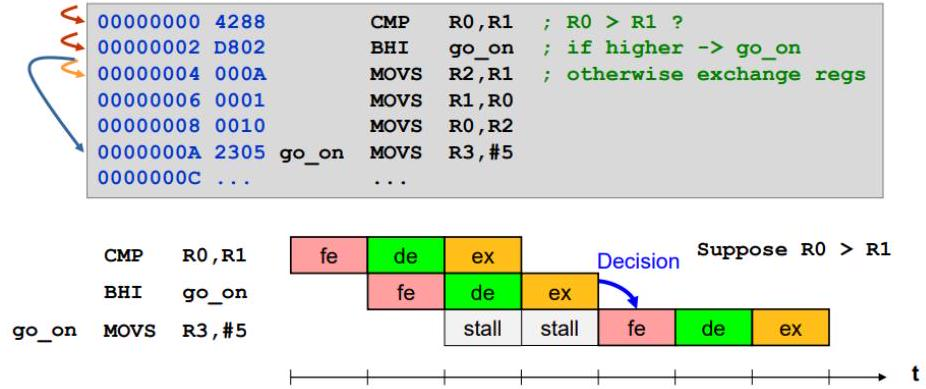
\includegraphics[width=\linewidth]{images/2024_12_29_79e6b22f503fb7b4f718g-15}

\textbf{Optimization Techniques:}
\begin{itemize}
  \item Branch prediction based on history
  \item Instruction prefetch
  \item Out-of-order execution
\end{itemize}

\textbf{Optimization Limits:}
\begin{itemize}
  \item Security vulnerabilities (Meltdown, Spectre)
  \item Complex optimizations increase risk
\end{itemize}
\end{concept}

\begin{concept}{Parallel Computing}\\
Different approaches to parallelism:
\begin{itemize}
  \item \textbf{Vector Processing}: Single instruction processes multiple data
  \item \textbf{Multithreading}: Multiple threads share CPU
  \item \textbf{Multicore}: Multiple CPU cores on one chip
  \item \textbf{Multiprocessor}: Multiple CPUs in system
\end{itemize}
\end{concept}

\begin{KR}{Optimizing System Performance}\\
Steps for performance optimization:
\begin{enumerate}
  \item Analyze performance bottlenecks
  \item Choose appropriate architecture:
    \begin{itemize}
      \item RISC vs CISC based on application
      \item Consider memory architecture
    \end{itemize}
  \item Implement pipelining:
    \begin{itemize}
      \item Balance stage delays
      \item Handle hazards appropriately
    \end{itemize}
  \item Consider parallelization options
  \item Evaluate security implications
\end{enumerate}
\end{KR}